\documentclass{article}
\usepackage{graphicx, amsmath}
\graphicspath{ {./images/} }

\title{Ch. 5 Optional -- Solns}
\author{Principles of Microeconomics}
\date{\today}

\begin{document}

\maketitle

\begin{enumerate}

\item

	\begin{enumerate}
	
	\item $\eta = \left| \frac{-12\%}{10\%} \right| = 1.2$
	
	\item 
		\begin{gather*}
		0.5 = \left| \frac{\% \Delta Q_D}{-20\%} \right| \\
		10\% = \% \Delta Q_D
		\end{gather*}
		Note: $\% \Delta Q_D$ is positive because of the law of demand. If price decreases, quantity demanded increases.
		
	\item 
		\begin{gather*}
		1 = \left| \frac{-15\%}{\% \Delta P} \right| \\
		\% \Delta P = 15\%
		\end{gather*}
		Note: $\% \Delta P$ is positive because of the law of demand. If quantity demanded decreases, that means price must have increased.
		
	\item
		\begin{gather*}
		1.2 = \frac{\% \Delta Q_S}{10\%} \\
		12\% = \% \Delta Q_S
		\end{gather*}
		Note: $\% \Delta Q_S$ is positive because of the law of supply. If price increases, quantity supplied increases.
		
	\item $P.E.S = \frac{-10\%}{-15\%} = 0.67$
	
	\end{enumerate}
	
\newpage
	
\item

	\begin{enumerate}
	
	\item I would not. Since demand is elastic, an increase in price will decrease quantity significantly. Quantity demanded will drop proportionately more than price will increase, so total revenue will decrease.
	
	\begin{center}
	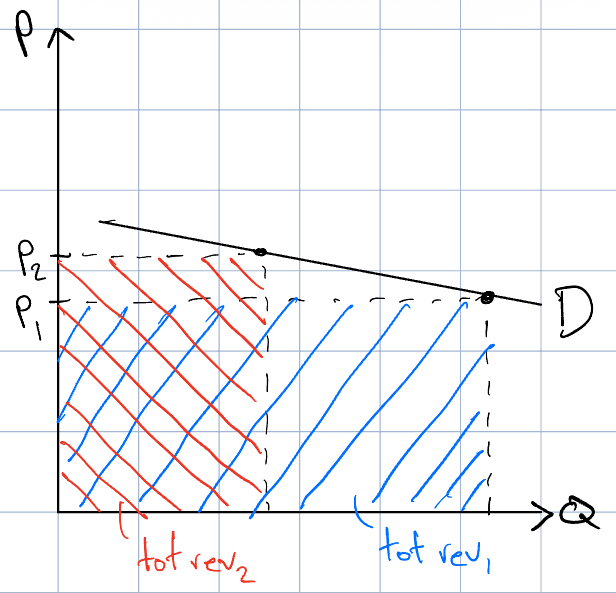
\includegraphics[width = 0.5\textwidth]{problem2a}
	\end{center}
	
	\item I would not. Since demand is inelastic, a decrease in price will not increase quantity significantly. Quantity demanded will increase proportionately less than price will decrease, so total revenue will decrease.
	
	\begin{center}
	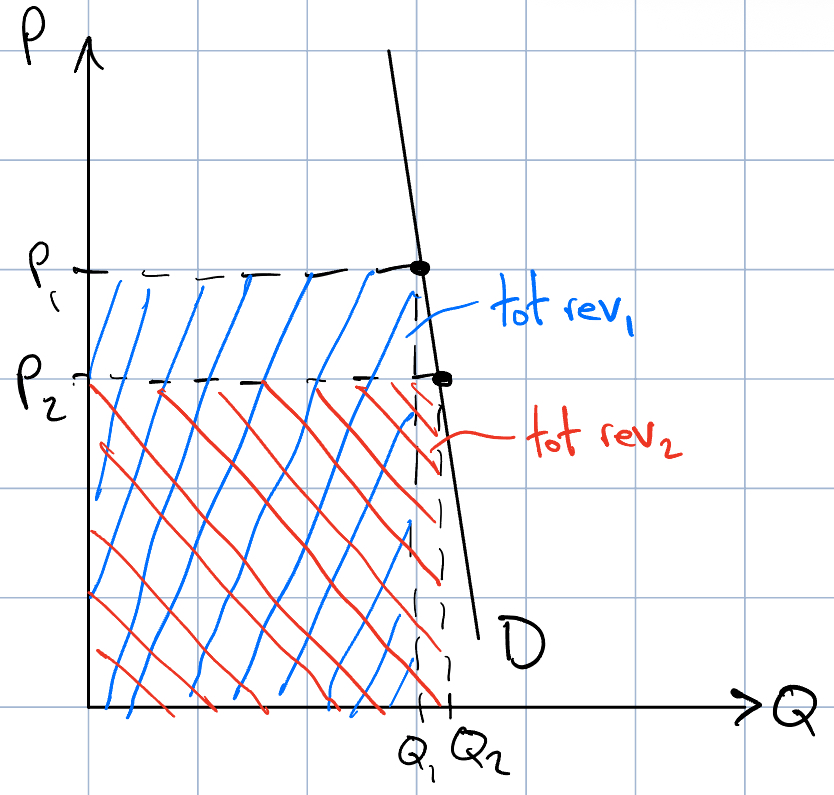
\includegraphics[width = 0.5\textwidth]{problem2b}
	\end{center}
	
	\end{enumerate}

\newpage
	
\item

	\begin{enumerate}
	
	\item I disagree. Since demand is inelastic, an increase in price won't decrease quantity significantly. The increase in price will be proportionately larger than the decrease in quantity, so total revenue will go up. That means buyers will spend more on cocaine.
	
	\begin{center}
	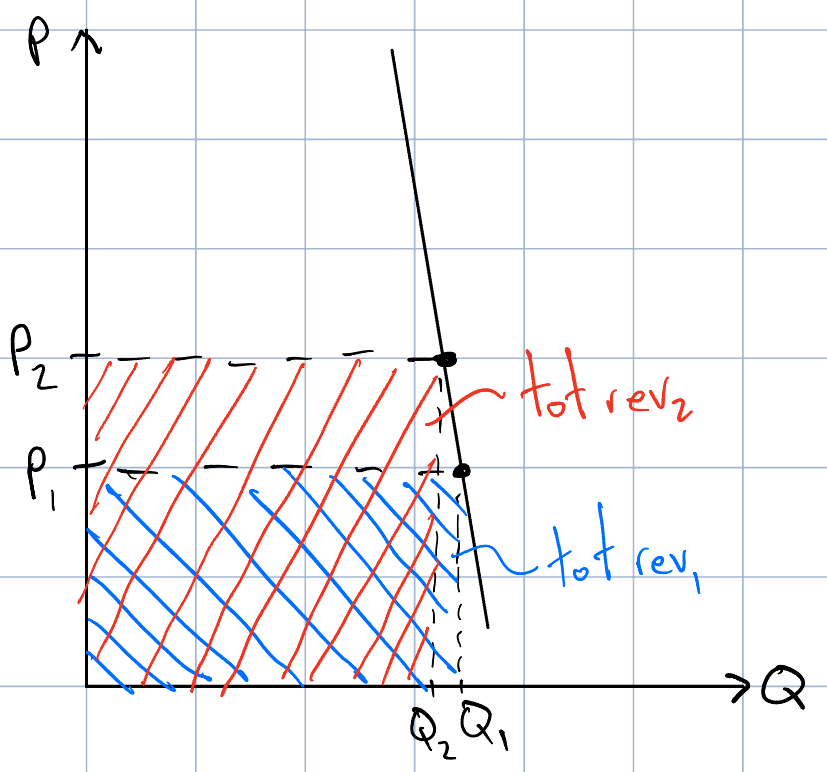
\includegraphics[width = 0.5\textwidth]{problem3a}
	\end{center}
	
	\item I disagree. Since demand is elastic, a decrease in price will increase quantity significantly. The decrease in price will be proportionately smaller than the increase in quantity, so total revenue will go up.
	
	\begin{center}
	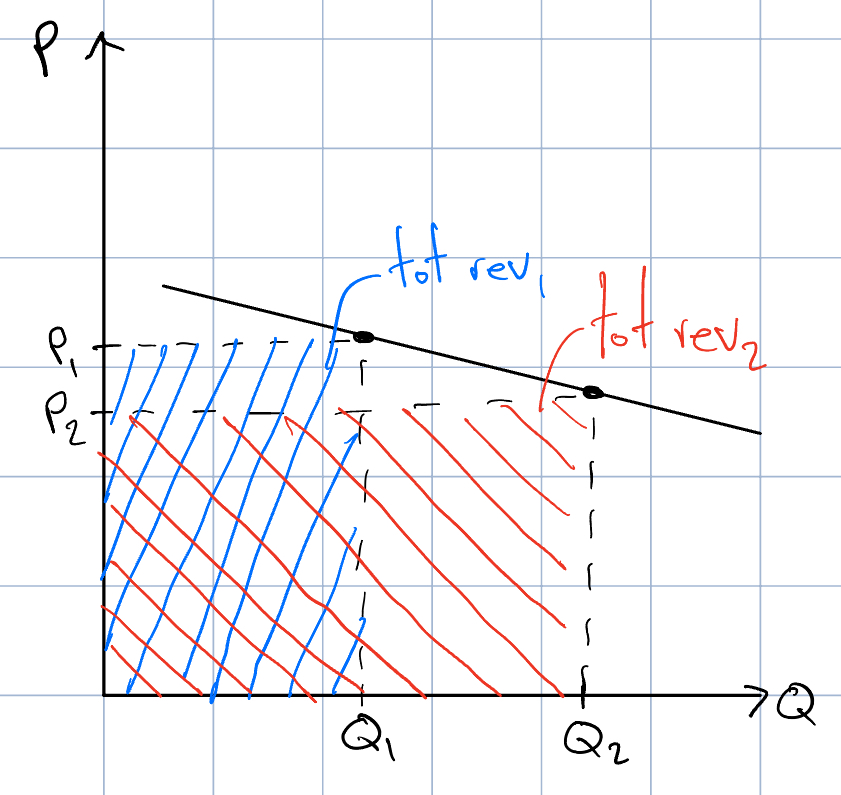
\includegraphics[width = 0.5\textwidth]{problem3b}
	\end{center}
	
	\newpage
	
	\item I disagree. If demand is unit elastic, then an increase in price leads to a proportionate decrease in quantity. The increase in price is offset by the decrease in quantity, so revenue stays the same. 
	
	\begin{center}
	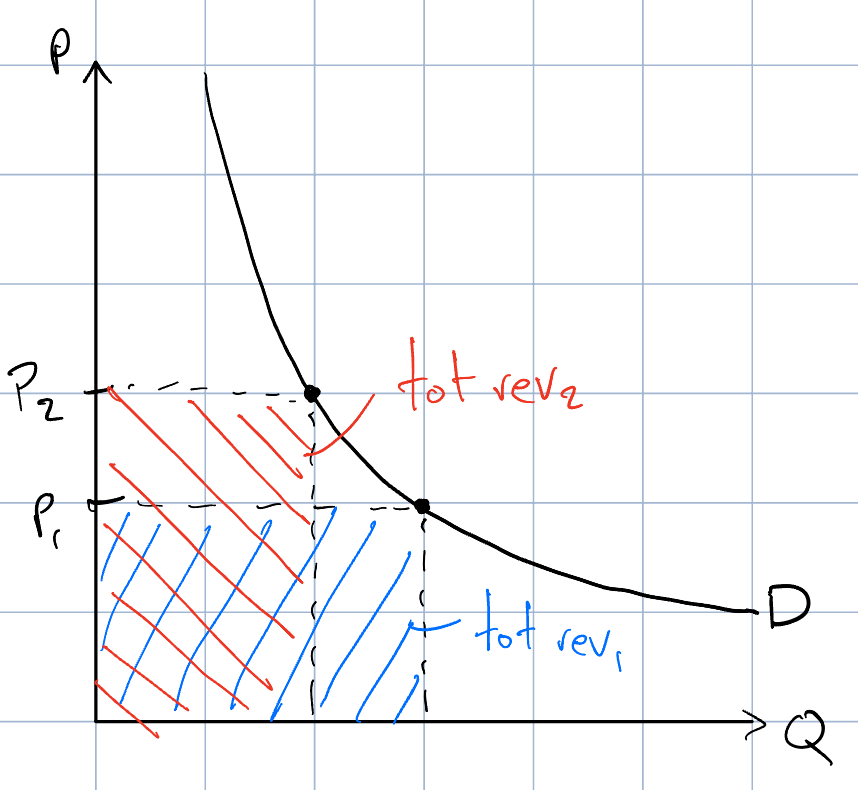
\includegraphics[width = 0.5\textwidth]{problem3c}
	\end{center}
	
	\end{enumerate}
	
\item Let $x = \% \Delta Q_D$.
	\begin{gather*}
	1.05PQ = 1.1P*(1 + x)Q \\
	1.05PQ = 1.1(1+x)PQ \\
	1.05 = 1.1(1+x) \\
	\frac{1.05}{1.1}-1 = x \\
	-0.05 = x
	\end{gather*}
	$Q_D$ decreased by 5\%.
	\begin{gather*}
	\eta = \left| \frac{-0.05}{0.10} \right| \\
	\eta = 0.5
	\end{gather*}
	Demand is inelastic because $\eta = 0.5$. Taxicab drivers were assuming that demand was perfectly inelastic. For a 10\% increase in price to cause a 10\% increase in revenue, the quantity demanded would have to remain constant despite the change in price. Quantity demanded only remains constant despite changes in price when demand is perfectly inelastic.
	
\item
	\begin{itemize}
	
	\item Products A \& B are complements because their cross-price elasticity of demand is negative. That means when the price of one goes up, the quantity demanded of the other goes down -- the definition of complements.

	\item Products C \& D are substitutes because their cross-price elasticity of demand is positive. That means when the price of one goes up, the quantity demanded of the other goes up -- the definition of substitutes.
	
	\item Products E \& F are unrelated because their cross-price elasticity of demand is zero. That means when the price of one goes up, the quantity demanded of the other doesn't change.
	
	\end{itemize}

\end{enumerate}

\end{document}